\label{enhancement}
% Let consider an example, we have an application with four computing functions and only implement 2 kernels written for the first function and the third one to be executed on coprocessor. As described in Fig. \ref{fig:working mechanism}, to execute the first function, data must be transfered to the coprocessor first and then taken back to host CPU after computation to be input for the second function. This process is repeated for the last two functions. We can see that, this application transfers data to coprocessor two times, and take it back to CPU times. However, data transferring leads to depletion in performance. Therefore, to minimize transferring time in this application, all functions must have corresponding kernels written to be offloaded to coprocessor. With this approach no matter there are how many functions in an application, we only spend one time to send data to coprocessor and one time to take the result back when all functions has finished. 

% In the previous PyMIC version, it only provides several functions to initialize, change data in array and some simple operations on array such as add, subtract, multiply, and so on. In this paper, we enhance PyMIC by implementing all unit functions that mainly support for deep learning applications with high performance so that users do not have to spend time writing their own kernel. Our kernels are written in C code and parallelized by using OpenMP frameworks to make use of computing power of Intel Xeon Phi. Each unit function is implemented and designed in 3 steps:

% \begin{itemize}
% \item Defining function prototype for C kernel: In this step, we identify parameters needed to be input of a kernel, and their data types. Each parameter is a piece of data transferred to coprocessor; therefore, the number of parameters needs to be chosen wisely to achieve the best performance.

% \item Implementing function in Python layer: function prototype in Python layer is the same as the one of Numpy so that users can easily use PyMIC in an application using Numpy if they want to execute their application on coprocessor without much modification because their function APIs are the same. The functionality of functions in this layer is to prepare parameters defined in previous step to transfer to kernels in C layer  		
			
% \item Implementing function in C layer: After receiving input data from Python layer, C functions will do computation depending on input data types and return data back to Python layer. These kernels use data parallel algorithms which are implemented using \textbf{\#pragma omp simd} to take advantage of vector units, and \textbf{\#pragma omp for} to use up all core in Intel Xeon Phi
% \end{itemize}

By improving pyMIC, developers can save time and effort developing high-level applications. To be specific, we modify the existing functions, provide more compute functions, and features to increase the flexibility of pyMIC. All of the functions are parallelized by using OpenMP frameworks \cite{openmp}. Besides, the reason we use OpenMP is because of its simplicity and fine-grained control over other frameworks such as Intel Cilk or TBB. Moreover, because of most operations on arrays are element-wise, data parallel algorithms that use OpemMP achieve better performance than the other two \cite{tousimojarad2014comparison}. In summary, we make the following modifications:

\begin{itemize}
\item The first improvement of pyMIC is that it now can fully support basic data types in both C and Python, which therefore increases the flexibility of pyMIC to work well with applications that require high precision (float 64 bits)[] or low precision (float 32 bits) []. In order to understand data types of data transfered to C kernels from Python layers, pyMIC has a mechanism of mapping data types to specific integers which are described in details in Table \ref{table : data type mapping}. To be specific, in each data type, there will be a unique integer to represent for that type. With the present of the integer, compute kernels now know how to process data corresponding with that data types. Moreover, many other data types such as string or char can also be added easily in the next versions.

\begin{table}
\centering
\caption{Mapping data types in pyMIC.}
\label{table : data type mapping}
% \begin{tabular}{ |P{3cm}|P{3cm}|P{3cm}|  }
\begin{tabular}{ |c|c|c|  }
\hline
\textbf{Python} & \textbf{C} & \textbf{Integer value} \\ \hline
numpy.int64 & int64\_t &0 \\
numpy.int32 & int32\_t &1 \\
numpy.float64 & double &2 \\
numpy.complex128 &complex &3 \\
numpy.uint64 & uint64\_t & 4\\
numpy.float32 & float & 5\\
numpy.bool & bool & 6\\
\hline
\end{tabular}

\end{table}

\item Secondly, operations that require two arrays as input now can be applied on two arrays with different data types. Previously, pyMIC only supports operations for two input arrays with the same data types. When two input arrays have different data types, data types of the output array will follow the following rules in Table \ref{table : Convert Rule}. Among two input data types, the one that has higher priority will the data type of output array. The priority is depicted in Table \ref{table : Data Type Rank}. Our method is based on type conversion in C and Python language to prevent data loss.

\begin{table}
\centering
\caption{Data types of output array for two input array with different data types.}
\label{table : Convert Rule}
 %\begin{tabular}{ |P{3cm}|P{3cm}|P{3cm}|  }
 \begin{tabular}{ |c|c|c|  }
\hline
\textbf{Array A} & \textbf{Array B} &  \textbf{Array C}\\
\hline

int32	&	int64	&	int64 \\
int32	&	float32	&	float32\\
int32	&	float64	&	float64\\
\hline
int64	&	int32	&	int64	\\
int64	&	float32	&	float32\\
int64	&	float64	&	float64\\
\hline
float32	&	int32	&	float32\\
float32	&	int64	&	float32\\
float32	&	float64	&	float64	\\
\hline
float64	&	int32	&	float64\\
float64	&	int64	&	float64\\
float64	&	float32	&	float64\\
\hline
\end{tabular}
\end{table}

\begin{table}
\centering
\caption{Priority of data types.}
\label{table : Data Type Rank}
 %   \begin{tabular}{ |P{4cm}|P{4cm}|  }
\begin{tabular}{ |c|c|  }
\hline
\textbf{Data type} & \textbf{Priority} \\
\hline
numpy.float64 & 1\\
numpy.float32 & 2 \\
numpy.int64 & 3 \\
numpy.int32 & 4\\
numpy.bool & 5\\

\hline
\end{tabular}
\end{table}

\item Additionally, we also modify the existing functions of pyMIC to achieve better performance and more flexible. Specifically, we parallelize all compute functions of pyMIC such as function add, sub, and mul two arrays by means of vectorization and multithreading. The experimental results will be mentioned in Section \ref{sec:function_eval} Furthermore, function add, sub, mul previously only support applying on 2 arrays with the same shapes or between an array and a scalar number. Now, they can support applying on 2 arrays with different shapes by using broadcasting. In NumPy, the term broadcasting describes how NumPy treats arrays with different shapes during arithmetic operations \cite{Broadcast}. For example, array b with smaller shape will be stretched during the arithmetic operation into an array with the same shape as a (Fig \ref{fig:Broadcasting}). 

\begin{figure}[]
\centering
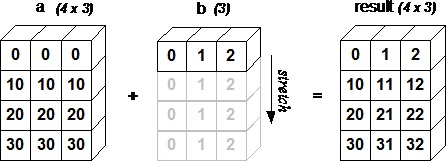
\includegraphics[scale=0.5]{img/broadcast.jpg}
\caption{Broadcasting in NumPy}
\label{fig:Broadcasting}
\end{figure}

\item Next, to be more flexible, pyMIC also supports advanced indexing for an array a with selection object obj \cite{AdvancedIndexing}. It is triggered when the command a[obj] is called, a new array containing selected values will be returned. For instance in Fig \ref{fig:advanced-indexing}, we want to select two values at two top corners of 2-d array, a selection object obj with value [[0, 1], [0, 2]] will be created to index array a. However, for now we only support advanced indexing for 2-d arrays and selection object with integer values.

\begin{figure}
    \centering
    \begin{lstlisting}
>>> a
array([[1, 2, 3],
       [4, 5, 6]])
>>> obj = [[0,0], [0,2]]
>>> a[obj]
array([1, 3])
\end{lstlisting}
    \caption{Example of advanced indexing}
    \label{fig:advanced-indexing}
\end{figure}

\item Finally, we also provide unit functions used to build high-level functions in deep learning such as activate function, loss function, accuracy function, and so forth, to swiftly form artificial neural networks. All of them are parallel and optimized so that they can fully take use of 512-vector registers and many cores in Intel Xeon Phi coprocessor. In Sect. \ref{sec:function_eval}, a list of all of the modified and added functions in pyMIC is listed.
\end{itemize}